%%%%%%%%%%%%%%%%%%%%%%%%%%%%%%%%%%%%%%
% START ADDING TEXT HERE 
%
% Feel free to use \include commands to structure text in smaller
% pieces 
% 
%%%%%%%%%%%%%%%%%%%%%%%%%%%%%%%%%%%%%%


% Abstract gives a brief summary of the main points of a paper:
\begin{abstract}
  This paper gives a brief overview of the use of pigeon as a physical
  layer underlying  the IP protocol. 
\end{abstract}

% the actual content, usually separated over a number of sections
% each section is assigned a label, in order to be able to put a
% crossreference to it

\section{Introduction}
\label{sec:introduction}

The introduction describes the problem, why it is important, the main
ideas of the following paper, what are the main contributions of the
paper, etc. 

% Note: for a SEMINAR, Related Work usually is a BAD idea and makes no
% sense! 
\section{Some section}
\label{sec:relwork}

Use section labels for references, e.g., to

Section~\ref{sec:introduction}, that offer competing solutions, etc.

All sources must be properly referenced, ideally by using the
BiBTeX/Biber system. References can then be very conveniently made
with the \texttt{\\cite} command. For example, reference
\cite{leuwen00:_handb_schol} discusses some of the elementary rules on
writing scientific papers, amongst others how to correctly cite other
documents.  Lot's of other sources exist to help with writing
\cite{williams16:_style} or research in general
\cite{booth16:_craft_resear}.

Reference~\cite{Taylor:SIGuide:95}, e.g., describes how to
correctly use the SI system of units and their correct typographical
representation.


\section{Some other section}
\label{sec:model}


Such a section could, among other things, include a figure. Note that
a figure is a so-called floating object: it is moved around the actual
text in order to best fit on a page. This is in stark contrast to some
GUI-based word processing tools, where the placement of figures is
usually more associated with luck than principle.

As figures float around, expressions like ``the following figure''
must never be used. Instead, figures need a caption, a label, and must
be properly referenced in the main text. An example for this concept
is shown in Figure~\ref{fig:example}. 

\begin{figure}[htbp]
  \begin{center}
    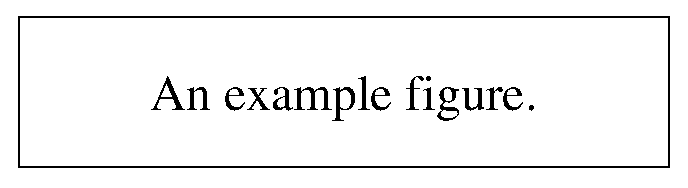
\includegraphics[width=\columnwidth]{example}
    \caption{An example figure with a caption.}
    \label{fig:example}
  \end{center}
\end{figure}

In general, only vector graphics in PDF or (possibly) encapsulated
postscript (eps) format should be included in any kind of text, as
this allows arbirary scaling, rotation etc.\ without any loss of
quality. Bitmap formats (PNG, JPEG, GIF, \dots) should only be used if no
other alternative exists --- e.g., when including photographs. 

\section{Word processing \& \LaTeX}
\label{sec:latex} 

This document has already introduced the most important constructs of
\LaTeX. What is necessary to produce documents with \LaTeX is simple
any normal text editor and a \LaTeX distribution. This is commonly
installed on practically all UNIX-type systems; for Windows, an
excellent \LaTeX exists, called MikTeX, available from
\url{www.miktex.org}. Almost all distributions come with a large patch
of examples and introductory material; consult your local installation
for details. 

Lots of supplementary and background information, FAQs, etc.\ is
available from the Comprehensive TeX Archive Network (CTAN); the
German mirror of which is \url{www.dante.de}. 


\section{Just some text}
\label{sec:just-some-text}

Just some text to show pagination etc. 

Pellentesque dapibus suscipit ligula.  Donec posuere augue in quam.  Etiam vel tortor sodales tellus ultricies commodo.  Suspendisse potenti.  Aenean in sem ac leo mollis blandit.  Donec neque quam, dignissim in, mollis nec, sagittis eu, wisi.  Phasellus lacus.  Etiam laoreet quam sed arcu.  Phasellus at dui in ligula mollis ultricies.  Integer placerat tristique nisl.  Praesent augue.  Fusce commodo.  Vestibulum convallis, lorem a tempus semper, dui dui euismod elit, vitae placerat urna tortor vitae lacus.  Nullam libero mauris, consequat quis, varius et, dictum id, arcu.  Mauris mollis tincidunt felis.  Aliquam feugiat tellus ut neque.  Nulla facilisis, risus a rhoncus fermentum, tellus tellus lacinia purus, et dictum nunc justo sit amet elit.

Nullam eu ante vel est convallis dignissim.  Fusce suscipit, wisi nec facilisis facilisis, est dui fermentum leo, quis tempor ligula erat quis odio.  Nunc porta vulputate tellus.  Nunc rutrum turpis sed pede.  Sed bibendum.  Aliquam posuere.  Nunc aliquet, augue nec adipiscing interdum, lacus tellus malesuada massa, quis varius mi purus non odio.  Pellentesque condimentum, magna ut suscipit hendrerit, ipsum augue ornare nulla, non luctus diam neque sit amet urna.  Curabitur vulputate vestibulum lorem.  Fusce sagittis, libero non molestie mollis, magna orci ultrices dolor, at vulputate neque nulla lacinia eros.  Sed id ligula quis est convallis tempor.  Curabitur lacinia pulvinar nibh.  Nam a sapien.

Aliquam erat volutpat.  Nunc eleifend leo vitae magna.  In id erat non orci commodo lobortis.  Proin neque massa, cursus ut, gravida ut, lobortis eget, lacus.  Sed diam.  Praesent fermentum tempor tellus.  Nullam tempus.  Mauris ac felis vel velit tristique imperdiet.  Donec at pede.  Etiam vel neque nec dui dignissim bibendum.  Vivamus id enim.  Phasellus neque orci, porta a, aliquet quis, semper a, massa.  Phasellus purus.  Pellentesque tristique imperdiet tortor.  Nam euismod tellus id erat.

\section{Math}
\label{sec:math}

\(a+b=\sqrt{c}\ = \int \sin(x) \mathrm{d}x \) 


\section{Tables}
\label{sec:tables}

Tables  like Table~\ref{tab:example}; they float and should be typeset using the booktabs package (see
documentation there). 


\begin{table}[htbp]
  \centering
  \begin{tabular}{ll}
    \toprule 
    a & b \\
    \midrule 
    c & d \\
    e & f \\
    \bottomrule
  \end{tabular}
  \caption{Example table}
  \label{tab:example}
\end{table}


\section{Pet peeves}
\label{sec:pet-peeves}

\subsection{Language/correctness}
\label{sec:orgheadline1}
\begin{itemize}
\item It is ``related work'' in the singular -- ``work'' is considered a non-countable noun here and hence takes no plural ``s''. Do not think of it as the collection of papers, each one a single ``work''. 
\item Punctuation: Typical punctuation errors occur with compound and complex sentences; in particular, when conjunctive adverbs are used. See here for details: \url{http://www.towson.edu/ows/sentences.htm}
\item Watch out for punctuation rules, in particular, punctuation of defining vs.\ non-defining relative clauses (e.g., ``bla, that'' is almost always wrong).
\item Check hyphenation rules, in particular, for compound attributes (\url{http://en.wikipedia.org/wiki/English_compound#Hyphenated_compound_adjectives}). Roughly: compound nouns tend not to be hyphenated, compound attributes usually are (with plenty of exceptions)
\item ``can not'' and ``cannot'' mean opposite things; often, many people  mean ``cannot'' but incorrectly write ``can not''. E.g., ``This dog can not bark'' (it is able to sometimes shut up) vs.\ ``This dog cannot bark'' (it is unable to produce sound).
\item It is ``et al.'', abbreviating ``et alia''; hence, the period is required after ``al'' and wrong after ``et''
\item Quoting a comma rule from \url{http://grammar.ccc.commnet.edu/grammar/commas.htm} :

  \begin{quote}
    Use a comma to set off introductory elements, as in ``Running
    toward third base, he suddenly realized how stupid he looked.''

    It is permissible to omit the comma after a brief introductory
    element if the omission does not result in confusion or hesitancy
    in reading. If there is ever any doubt, use the comma, as it is
    always correct. 
  \end{quote}
 If you would like some additional guidelines on 
    using a comma after introductory elements, click HERE.
\item Currently, an ``idiot's comma'' is sneaking into common language, offsetting a (perhaps long) subject from its predicate. This is \emph{totally and absurdly} wrong! 
\item The so-called ``zero article'' (leaving out any article from a noun
phrase) is well described here:
\url{http://grammar.ccc.commnet.edu/grammar/determiners/determiners.htm}
(search for ``zero article''); in context with abstract nouns, this
link might be a good start:
\url{http://www.bbc.co.uk/worldservice/learningenglish/youmeus/learnit/learnitv255.shtml}. Incorrect article use really hinders readability. 
\item Whether or not a word or an acronym is preceded by ``a'' or ``an'' depends on whether the initial \emph{sound} is a vowel or a consonant; the written form of word or acronym does not matter!

\item Watch out for correct use of third person singular ``s'' conjugation
\end{itemize}

\subsection{Style}
\label{sec:orgheadline2}
\begin{itemize}
\item Read and follow  \url{http://www.ieee.org/documents/stylemanual.pdf}
\item ``Section 4'', ``Figure 1'', \ldots{} are proper names and are hence capitalized; the word ``section'', ``figure'', \ldots{} WITHOUT the number does not refer to a specific entity, is hence not a proper name, and is hence not capitalized.
\item Avoid ``lonely'' headings -- if there is a 3.1, there must also be a 3.2
\item Use verbs, not adjectives. E.g., ``is dependent on'' $\rightarrow$ $depends on$ (same thing, shorter text)
\item Check rules on capitalization of title case, in particular, for conjuctions, prepositions, etc.
\item Do not use contractions: write ``does not'' instead of ``doesn't''; ``has not'' instead of ``hasn't'', etc.
\end{itemize}

\subsection{Typesetting}
\label{sec:orgheadline3}
\begin{itemize}
\item Use a short space $\backslash,$, between number and unit. It is ``2\,kg'', not ``2 kg'' (and certainly not ``2kg''). Never use ``sec''; the correct abbreviation for second is ``s''. In general, there are plenty of rules for units in the SI system; compare \url{http://physics.nist.gov/cuu/Units/}
\item Units are typeset upright (roman)
\item Multi-letter variables, subscripts etc.\ are typeset upright. Example: \(t_\mathrm{abc}\) would be correct. (only single-letter variables are italic)
\item There is a space between a word and a citation: it is ``bla [1]'',
  not ``bla[1]''. Also, the citation goes BEFORE the full stop, it is
  part of the sentence: ``bla bla [1].'' not: ``bla bla. [1]'' 

\item Distinguish between hyphen and dash ( - or -- in \LaTeX{}) -- this is REALLY annoying. 
\item In many fonts, the signs for opening quotes and closing quotes differ. \LaTeX{} allows the writer to express which ones are desired by ``   for opening quotes and ''  for closing quotes. Using "bla", however, is not correct! Single quotes are set correspondingly.  For languages other than English, there are specific quotation commands as well. (Any decent text preparation systems allows this distinction; consult your manual if you are not using \LaTeX{}.)
\item Correct rules for typesetting math and similar texts are collected
here: \url{http://physics.nist.gov/cuu/pdf/typefaces.pdf}
\url{http://physics.nist.gov/cuu/pdf/sp811.pdf}
\item \textbf{Never, ever} include bitmaps, especially not bitmaps with lossy
compression except for things like photpgrahs. Use vector formats like EMF, EPS, or PDF.
\end{itemize}

\subsection{References}
\label{sec:orgheadline4}
\begin{itemize}
\item BiBTeX: watch out for use of \{\} in title field to ensure correct capitalization
\item BibTeX: mind the warnings of BiBTeX! If BiBTeX complains about a missing field, it usually really is required!
\item When quoting a figure or a table, the caption should state the reference as well as which figure or table it is in the original reference
\end{itemize}

\subsection{Other resources}
\label{sec:orgheadline5}
\begin{itemize}
\item \url{http://www.ece.ucdavis.edu/~jowens/commonerrors.html}
\end{itemize}


\section{Conclusion}
\label{sec:concl}

At the end, there is a final section \emph{concluding} a paper,
putting the entire work into perspective and explaining, on a larger
level, what the consequences of this work are. Also, unexpected
results can be discussed here, etc.

Putting a \emph{summary} at the end is a common, yet bad practice. Try
to avoid it; it is just boring. 

 